\subsection{Tumor Radiation}

As mentioned in the previous section external tumor radiation is a widespread non-invasive modality for cancer treatment with or without tumor resection.
It is or should be used for over 50\% of all cancer patient once in the course of their illness \cite{delaney_role_2005}. 
The effectiveness of tumor radiation is based on the physical processes that cause biological damage to cells.
Interaction of photons and secondary electrons release free radicals inside the tissue, which cause \ac{DNA} damage in the form of single- or double strand breaks.
The tumor microenviroments conditions such as hypoxia, low pH and nutrient deficiency reparation mechanisms in tumor cells are down regulated compared to healthy tissue \cite{li_dna_2021}.
Since tumours are usually located in deeper regions of the body, it is unavoidable to irradiate healthy tissue as well. 
An example of a prostate tumor and its surrounding organs at risk is shown in \autoref{fig:prostate_oar}.
Photons attenuation is described by an exponential decay, meaning that a photon beam can not be entirely shielded.
This has crucial importance for the application of radio therapy for tumor irradiation.
Due to the infinite range of photons, healthy tissue which is located behind the tumor volume, with respect to the beam direction, is also inevitably irradiated.
The aim of a treatment plan optimization process is to achieve an optimal dose coverage over the entire target volume, while irradiating surrounding \acs{OAR} as little as possible.
Spefici margins for dose coverage of tumor volumes as well as \acs{OAR} are covered by the intitutional standard operating procedure, which is oriented on current literature and medical studies.
Therefore the planning software takes all delineated \acs{OAR} in consideration and defines a optimal dose distribution.
Optimizing the possible accelerator settings to achieve this dose distribution is the key step during treatment planning.
The use of different defined radiation angles in combination with changing \ac{MLC} shapes results in a sparing of \ac{OAR} while achieving a high dose area with steep dose gradients at the \ac{PTV}.
To further decrease the bad side effects of irradiation of healthy tissue the plan is fractionated.
In multiple sessions the tumor volume is irradiated benefiting from the increased reparation mechanisms of healthy tissue.
The time between fractions is carefully chosen giving healthy tissue to repair some of the damage while the cells inside the tumor volume do not have enough time to repair crucial \ac{DNA} damage resulting in a steady decrease of the tumor cell population.

\begin{figure}
    \centering
    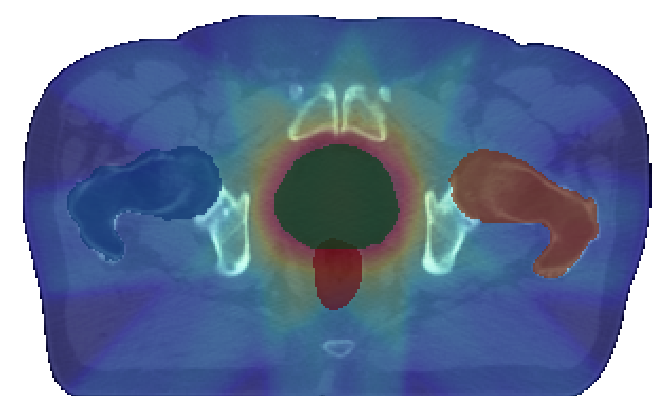
\includegraphics[width=0.5\textwidth]{example_image.pdf}
    \caption{
        CT image of a prostate caner patient including the dose distribution of the respective treatment plan. Areas of high dose deposition are displayed in red and orange. Left and right femur head aswell as rectum displayed in blue and orange and red respectively are displayed along the \acs{PTV} displayed in green.
        }\label{fig:prostate_oar}
\end{figure}

\subsection{MR Linear Accelerator}

Basis for the treatment planning is a conventional \acs{CT} taken as the first step in the treatment planning process.
Planning on this \acs{CT} is the base for each radiation session of all fractions.
For some entities whith moving organs such as sigmoid or bladder in the lower abdomen, this results in some uncertainties because it is assumed that the earliert aquired \acs{CT} still represents the position of the tumor volume aswell as the \acs{OAR}.
The Mr-Linac enables the aquisition of a MR image right before irradiation.
In combination with the provided pipeline that allows for fast treatment plan adaption to shifts and shape morphing of tumor volumes or \acs{OAR} these uncertainties can be reduced. 
The patient therefore receives a MR image before every fraction and the current treatmentplan is adapted based on the current positions and shapes of tumor and \acs{OAR}.
This is achieved by registration of the initial CT to the daily aquired MR image.
Delineations of tumor volumes aswell as \acs{OAR} are registered and the treatmentplan optionally adapted.\\
Current research is going towards the further exploration of opportunities involving the MR-Linac.
The vision behind the MR-Linac would be to adapt the treatment plan based on real-time image aquisition during the treatment.
To enable this protocol all involved steps in the treatment planning  pipeline need to be applicable in an MRI-only workflow, including delineation and dose deposition calculation.
MRI imaging is not a quantitative imaging modality, meaning that the pixel values of MRI images are not correlated to the electron density of the tissue represented by that tissue.
Dose deposition processes are dependant on particle energy aswell as tissue density.
Therefore a translation from qualitative MRI data to quantitative electron density imformation is needed to estimate deposited dose inside a volume.\\
An MRI only worklow is ultilately resulting in in-time adaption to intra-fraction movements such as unwanted patient movement aswell as breathing motion potentially leading to a significant decrease in safety margins, which are currently needed to account for unvertainties during treatment.\\
Multiple steps in the planning pipeline need to be applied in real-time, which is currently not possible due to high calculation intensity.
The estimation of dose deposition is a process that is involved in the step of iterative treatment plan optimization.
Currently state of the art for precise dose dopsition estimation is a \ac{MC} based solution.
Downside of \acs{MC} simulations is that they are very time consuming to achieve a sufficently accurate result.

\subsection{Physical Fundamentals}

The magnetic field which is present at all times inside the MR-linac has a strength of 1.5 Tesla.
Photons are not charged particles meaning that they are not affected by the magnet field.
Secondary electrons are created by interaction of photons with matter. 
Since electrons are charged particles they obey the Lorentz force as first described by \citeauthor{lorentz_versuch_1937} in \citeyear{lorentz_versuch_1937}~\cite{lorentz_versuch_1937}.  
Electrons are the main contributor to the dose deposition. 
Therefore results a change in trajectory of electrons also in a change in dose deposition along the Lorentz force.
Especially at the intersection of tissue to air cavities inside the human body the effect of the electric field is noticable.
It results in an increasing dose deposition on the surface of the tissue due to the \ac{ERE}.
The mean free pathlength of electrons is bigger in air resulting in an 180° degree turn of electrons and dose deposition at the tissue surface.\\
Base for the dose calculation algorithms in the form of \acs{MC} is that basics interaction processes of particles are quantitatively described.
The main contributing particles in the energy sectrum used at a linear accelerator are photons and electrons.
Photons interact with matter in the form of inelastic interaction such as compton scattering or the photoeffect. 
For both interaction processes the entire or partial energy from the photon is transfered to an electron of the interaction sight.
Due to the decreased mean free pathlength of electrons they deposit their entire energy in the directly surrounding tissue.
Interaction processes are of stochastic nature.
During the \acs{MC} simulation parameters such as free pathlength, interaction process, radiation angle after an interaction are determined by the prior knowledge of the probability distributions of these physical processes.


\subsection{Dose Calculation}

As previoulsy mentioned the main dose deposition algorithm we focus on is \acs{MC}.
There are multiple other dose deposition algorithms present in literature aswell as clinical use, such as collapsed cone \cite{ahnesjo_collapsed_1989} or pencil beam algorithms \cite{mohan_differential_1986} which is currently used as a primary dose estimation algorithms in the institutional planning software.\\
\acs{IMRT} treatment plans are composed of individual segments. 
A segment consists of a specific gantry angle, \acs{MLC} configuration and a predefined number of \ac{MU}.
The amount of radiated photons is measured in \acs{MU} and is measured in a constancy test for each linear accelerator.
Summation of the dose deposited from all segments with their respected \acs{MU} results in the dose distribution of the entire plan.\\
EGSnrc \cite{noauthor_nrc-cnrcegsnrc_2021} is a \acs{MC} based software tool which enables us to calculate dose distributions for single segments instead of the entire dose distribution of the plan, provided in the DICOM-dose file.
Required for an accurate dose estimation is an accurate model of the accelerator head.
Provided by previous work from \citeauthor{friedel_development_2019}~\cite{friedel_development_2019}, the head model implemented in EGSnrc was used to create distributions for single segments. 
Each segment simulated with the EGSnrc software tool is normed to 100 \ac{MU} which enables us to indivudually scale each segment to the radiated \ac{MU} listed in the DICOM-plan file. 

 
%     \item \textbf{Und dann auf Dosisdeposition eingehen / Was ist aktuelle Methode} hier noch viel verschieben nach material und methodik
%     \item (http://dx.doi.org/10.1118/1.2795842) monte carlo simulations are currently used for dose calculation for radiotreatment plans in a clinical setting. The interactions of photons in human tissue in the energy spectrum of interest for external beam therapy transfer the photon energy on to electrons or positrons. 
%these particles then transfer their energy into the surrounding tissue. before energy deposition the photon and especially the electron undergo a number of elastic and non elsatic interactions with atoms. In the process the main energy loss is caused by inelastic collisions and radiative interactions. the collisions result in ionization and therefore secondary electrons. radative interactions result in a energy trasnfer back to photons. the sum of these phenomena in a photon field results in a coupled electron-photon shower, which can be described by a coupled set of integrodifferntial transport equations. 
%due to the lack of a analystical solution, without any major simplifications and assumptions for conditions, the monte carlo algorithm is used to simululate a multitude of particle histories in the desired target volume. partical histories describe the exact way of a photon from the source to its point in the volume were it has lost all of its energy including enery transport to secondary electrons in the process of collisions. 
%the stochastic nature of the interaction processes of photons and electrons need for a large number of simulated particles to achieve an accurate result of dose deposition. the entirety of all simulated particles then results in an accurate dose distribution which can be used for treatment planning. the need for particle histories in the magnitude of 10\textsuperscript{7} to 10\textsuperscript{11} for accurate dose estimations, result in long simulation times. 

%deep learning is a prefered tool due to its short inference times aswell as super human performance level on certain tasks. the implementation of the fully convulitional network (https://arxiv.org/pdf/1411.4038.pdf) and its further development of the U-Net utilizing data from higher level representations of the data in the form of skip connections (https://arxiv.org/abs/1505.04597) have revolutionized the application of deep learning for image data and 3d data i the form of a 3D-UNets. 
    
%     \item Was ist die Contribution / Aims <- Ziel: Dosisvorhersage mit DL, möglichst robust
%     \item In this paper we investiage the capabilities of deep learning in the field of dose predictions for radio treatment plans. we aimed to achieve a robust dose prediction irrespective of the body region of interest and irresprective of the complexity of the treatment plan.
%     \item 
% \end{itemize}

% Show why Radiotherapy is so important: search for sources of application of radiotherapy for different entities. Prostate: \cite{geinitz_3d_2005, nguyen_curative_2005, budiharto_external_nodate} Mamma: \cite{ragaz_adjuvant_1997, lena_combined_nodate, taylor_estimating_2017} Head \& Neck: \cite{datta_head_1990, 
%bhide_advances_2010, castadot_adaptive_2010, morgan_adaptive_2020} Liver: \cite{hoyer_radiotherapy_2012, wulf_stereotactic_2001, wulf_stereotactic_2006, sterzing_stereotactic_2014, witt_mri-guided_2020} Lymph Nodes: \cite{degro_degro_2014, matsushita_stereotactic_2018, mikell_postoperative_2015, lundstedt_long-term_2012, jereczek-fossa_is_2015}

% Was ich noch brauche: Infos über MR-Linac, was ist die Vision hinter dem MR Linac (online adaption) 

% The use of Magnet Resonace Imaging (MRI) during radiotherapy has opened a variety of new opportunities for treatment optimization. MRI provides a better contrast in soft tissue areas of the body, compared to conventional computed tomograpy (CT), and can be used to assess functional image data from the patient in real time. 
%The enhanched contrast leads to better organs at risk (OAR) and tumor volume delineation. (doi:10.1016/S0360-3016(03)01446-9). Recent research efforts are exploring the capabilities of the hybrid MRI linear accelerator (MRI-Linac) (doi:10.1007/s00066-018-1386-z, doi:10.1016/j.radonc.2007.10.034,  doi:10.1002/acm2.12233). 
%The introduction of the MRI-Linac has transformed the clinical workflow for radiotherapy as well as treatment planning. Patients are required to receive one CT for initial treatment planning. For radiation in each fraction, the inital plan is registrated on the current MRI and optionally adapted to shift or size variation of the tumor volume (doi:10.1016/j.ctro.2019.04.001). Goal is to reach an MRI-only-workflow where image acquisition, treatment planning and radiotherapy only involve the MRI-Linac. 
%To achieve this goal multiple steps in the clinical workflow need to be adapted

% behind MRI Linac is an radiotreatment adaption in an onine manner, meaning that a shift of the tumor volume and changes to the patients anatomy due to movement can be considered to adapt the treatmentplan. This results in smaller safety margins (doi:10.1102/1470-7330.2004.0054) for tumor volumes and ultimately result in a lower delivered dose to organs at risk. To achieve this ultimate goal, multiple steps, such as anatomy segmentation, treatmentplan adaption and dose deposition simulations need to be able to be performed in real-time. 

% Welche besonderheiten gibt es bei einem MR-Linac im Vergleich zu einem normalem Bestrahler (Stichworte: ERE, Electron Deposition Shift)
% Wie funktioniert normale Dosisberechung (Monte Carlo doi:10.1118/1.598917), warum ist der Nutzen davon limitiert wenn man in die online Adaption möchte. 

% However, since MC simulation is a stochastic process, the resulting dose map contains inherent quantum noise whose variance is inversely proportional to the number of the simulation histories and, accordingly, to the simulation time. Typically, achieving clinically acceptable precision requires hours of CPU computation time. Graphics processing unit (GPU)-based parallel computation frameworks can accelerate MC simulation to a few minutes for a typical IMRT/VMAT plan (doi:10.1088/0031-9155/55/11/006)

% However, several areas in the clinical workflow require real-time dose calculation, such as inverse optimization of the treatment planning process for IMRT and VMAT (doi:10.1088/2632-2153/abdbfe)
% especially online radiotherapy and online plan adaption are limited by the time needed to recalculate dose distributions of beam settings and patient anatomies due to moving organs (doi:10.1016/j.clon.2018.08.001)


% Machine Learning Teil: Wie wird Machine Learning in verschiedenen bereichen der bestrahlungsplanung bezüglich MRI genutzt:
% Eine Implementierung und Nutzung dieser könnte zum Erreichen einer Online-Bestrahlnugsadaption führen

% 1. Autosegmentation (\cite{kazemifar_segmentation_2018, liang_deep-learning-based_2019}) aswell as uncertrainty (\cite{shen_medical_2019})

% 2. Radio Treatment Plan optimization (\cite{fan_automatic_2019, liu_deep_2019})

% 3. Dose Estimation (\cite{kontaxis_deepdose_2020, bai_deep_2021} active denoising of lower history MC Simulations (doi:10.1002/mp.13856 ))

% 4. Pseudo CT (\cite{han_mr-based_2017, wolterink_deep_2017, dinkla_mr-only_2018})
